\subsection{$\mu$+jets Channel}
\label{app:DataMCControlMUON}

%%%%%%%%%%%%%%
%%%%%%%%%%%%%%
% 6jetin
%%%%%%%%%%%%%%
%%%%%%%%%%%%%%
%\clearpage
%%%%%%%%%%%%%%
\begin{figure}[htbp]
\begin{center}
\begin{tabular}{ccc}
%
\includegraphics[width=0.30\textwidth]{figures/ht700SimpleBlindingCut/sysband_scaledAlpgen/LepPt_MUON_6jetin0btagex_NOMINAL.eps} &
\includegraphics[width=0.30\textwidth]{figures/ht700SimpleBlindingCut/sysband_scaledAlpgen/LepEta_MUON_6jetin0btagex_NOMINAL.eps} &
\includegraphics[width=0.30\textwidth]{figures/ht700SimpleBlindingCut/sysband_scaledAlpgen/MET_MUON_6jetin0btagex_NOMINAL.eps} \\
\includegraphics[width=0.30\textwidth]{figures/ht700SimpleBlindingCut/sysband_scaledAlpgen/Wlep_MassT_MUON_6jetin0btagex_NOMINAL.eps} &
\includegraphics[width=0.30\textwidth]{figures/ht700SimpleBlindingCut/sysband_scaledAlpgen/JetPt1_MUON_6jetin0btagex_NOMINAL.eps} &
\includegraphics[width=0.30\textwidth]{figures/ht700SimpleBlindingCut/sysband_scaledAlpgen/JetEta1_MUON_6jetin0btagex_NOMINAL.eps} \\
\includegraphics[width=0.30\textwidth]{figures/ht700SimpleBlindingCut/sysband_scaledAlpgen/Njets25_MUON_6jetin0btagex_NOMINAL.eps}  &
\includegraphics[width=0.30\textwidth]{figures/ht700SimpleBlindingCut/sysband_scaledAlpgen/HTHad_MUON_6jetin0btagex_NOMINAL.eps}  &
\includegraphics[width=0.30\textwidth]{figures/ht700SimpleBlindingCut/sysband_scaledAlpgen/HTAll_MUON_6jetin0btagex_NOMINAL.eps}  \\

\end{tabular}\caption{\small {Comparison between data and prediction in the $\mu$+jets channel in the control sample
with $\geq 6$ jets and $=0$ $b$-tagged jets  for a number of kinematic
variables. From top to bottom and left to right, the variables displayed are: lepton $\pt$, lepton $\eta$, missing transverse energy, $W$ transverse mass,
leading jet $\pt$, leading jet $\eta$,  $\hthad$ and $\HT$. The shaded area represents the total background uncertainty.}}
\label{fig:MUON_6jetin_0btagex}
\end{center}
\end{figure}
%%%%%%%%%%%%%%

\clearpage
%%%%%%%%%%%%%%
\begin{figure}[htbp]
\begin{center}
\begin{tabular}{ccc}
%
\includegraphics[width=0.30\textwidth]{figures/ht700SimpleBlindingCut/sysband_scaledAlpgen/LepPt_MUON_6jetin1btagex_NOMINAL.eps} &
\includegraphics[width=0.30\textwidth]{figures/ht700SimpleBlindingCut/sysband_scaledAlpgen/LepEta_MUON_6jetin1btagex_NOMINAL.eps} &
\includegraphics[width=0.30\textwidth]{figures/ht700SimpleBlindingCut/sysband_scaledAlpgen/MET_MUON_6jetin1btagex_NOMINAL.eps} \\
\includegraphics[width=0.30\textwidth]{figures/ht700SimpleBlindingCut/sysband_scaledAlpgen/Wlep_MassT_MUON_6jetin1btagex_NOMINAL.eps} &
\includegraphics[width=0.30\textwidth]{figures/ht700SimpleBlindingCut/sysband_scaledAlpgen/JetPt1_MUON_6jetin1btagex_NOMINAL.eps} &
\includegraphics[width=0.30\textwidth]{figures/ht700SimpleBlindingCut/sysband_scaledAlpgen/JetEta1_MUON_6jetin1btagex_NOMINAL.eps} \\
\includegraphics[width=0.30\textwidth]{figures/ht700SimpleBlindingCut/sysband_scaledAlpgen/Njets25_MUON_6jetin1btagex_NOMINAL.eps}  &
\includegraphics[width=0.30\textwidth]{figures/ht700SimpleBlindingCut/sysband_scaledAlpgen/HTHad_MUON_6jetin1btagex_NOMINAL.eps}  &
\includegraphics[width=0.30\textwidth]{figures/ht700SimpleBlindingCut/sysband_scaledAlpgen/HTAll_MUON_6jetin1btagex_NOMINAL.eps}  \\

\end{tabular}\caption{\small {Comparison between data and prediction in the $\mu$+jets channel in the control sample
with $\geq 6$ jets and $=1$ $b$-tagged jets  for a number of kinematic
variables. From top to bottom and left to right, the variables displayed are: lepton $\pt$, lepton $\eta$, missing transverse energy, $W$ transverse mass,
leading jet $\pt$, leading jet $\eta$,  $\hthad$ and $\HT$. The shaded area represents the total background uncertainty.}}
\label{fig:MUON_6jetin_1btagex}
\end{center}
\end{figure}
%%%%%%%%%%%%%%

\clearpage
%%%%%%%%%%%%%%
\begin{figure}[htbp]
\begin{center}
\begin{tabular}{ccc}
%
\includegraphics[width=0.30\textwidth]{figures/ht700SimpleBlindingCut/sysband_scaledAlpgen/LepPt_MUON_6jetin2btagex_NOMINAL.eps} &
\includegraphics[width=0.30\textwidth]{figures/ht700SimpleBlindingCut/sysband_scaledAlpgen/LepEta_MUON_6jetin2btagex_NOMINAL.eps} &
\includegraphics[width=0.30\textwidth]{figures/ht700SimpleBlindingCut/sysband_scaledAlpgen/MET_MUON_6jetin2btagex_NOMINAL.eps} \\
\includegraphics[width=0.30\textwidth]{figures/ht700SimpleBlindingCut/sysband_scaledAlpgen/Wlep_MassT_MUON_6jetin2btagex_NOMINAL.eps} &
\includegraphics[width=0.30\textwidth]{figures/ht700SimpleBlindingCut/sysband_scaledAlpgen/JetPt1_MUON_6jetin2btagex_NOMINAL.eps} &
\includegraphics[width=0.30\textwidth]{figures/ht700SimpleBlindingCut/sysband_scaledAlpgen/JetEta1_MUON_6jetin2btagex_NOMINAL.eps} \\
\includegraphics[width=0.30\textwidth]{figures/ht700SimpleBlindingCut/sysband_scaledAlpgen/Njets25_MUON_6jetin2btagex_NOMINAL.eps}  &
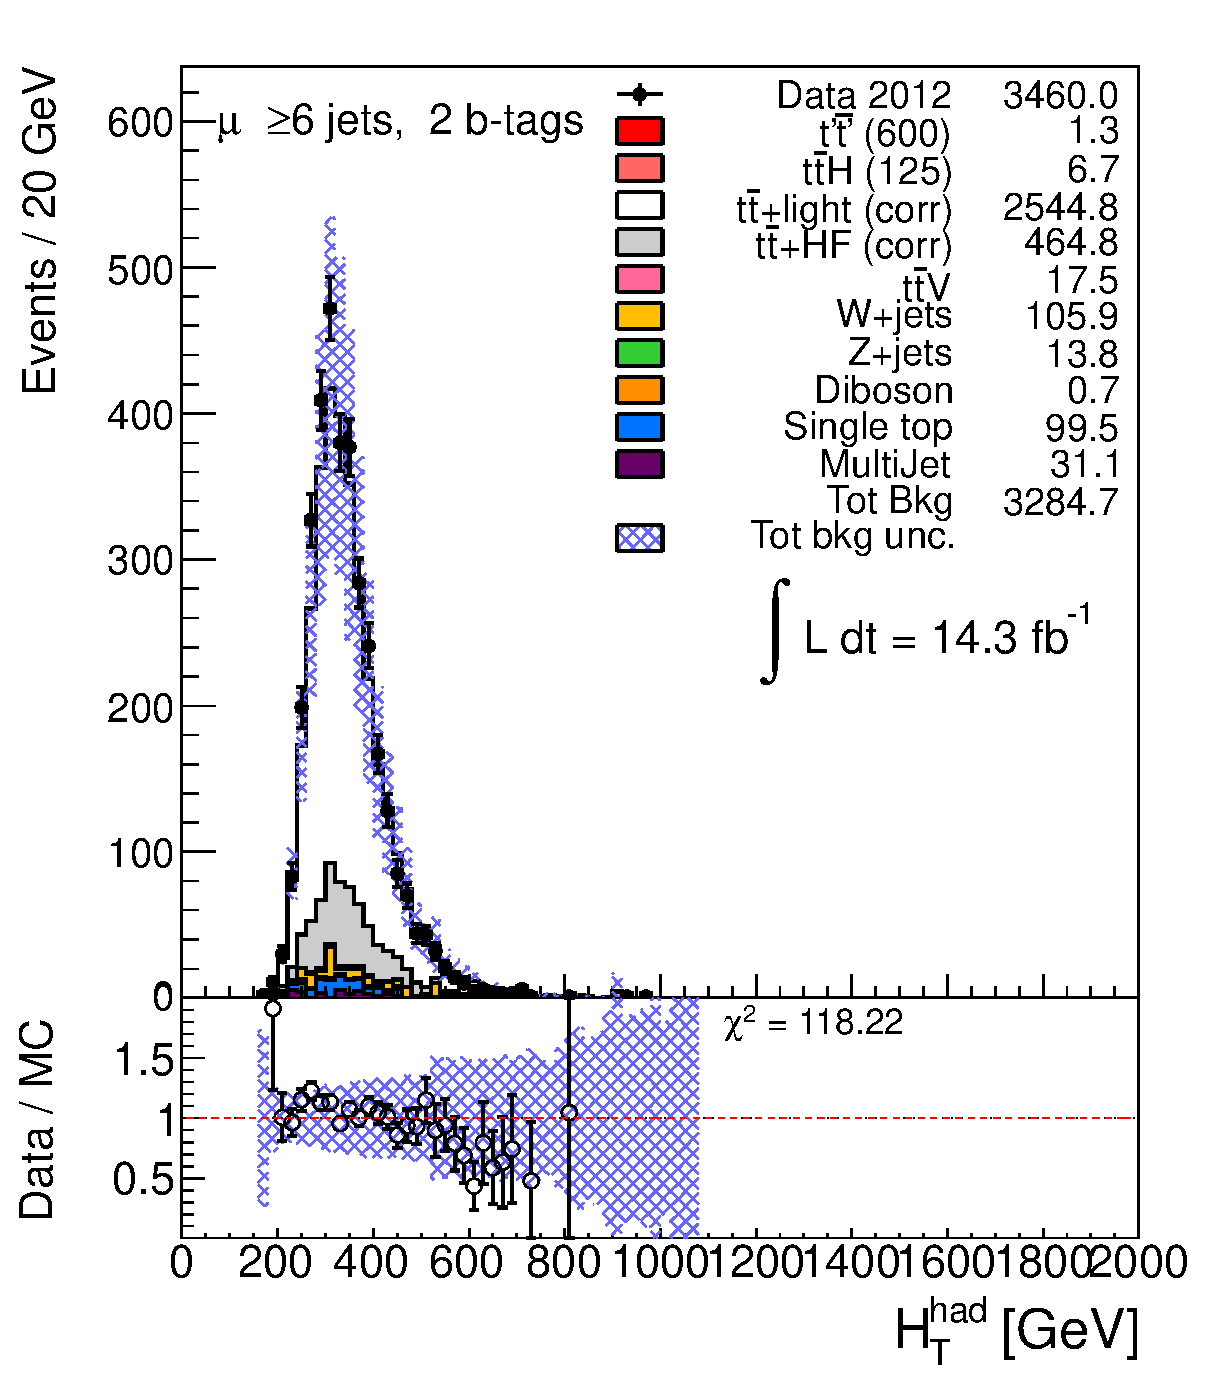
\includegraphics[width=0.30\textwidth]{figures/ht700SimpleBlindingCut/sysband_scaledAlpgen/HTHad_MUON_6jetin2btagex_NOMINAL.eps}  &
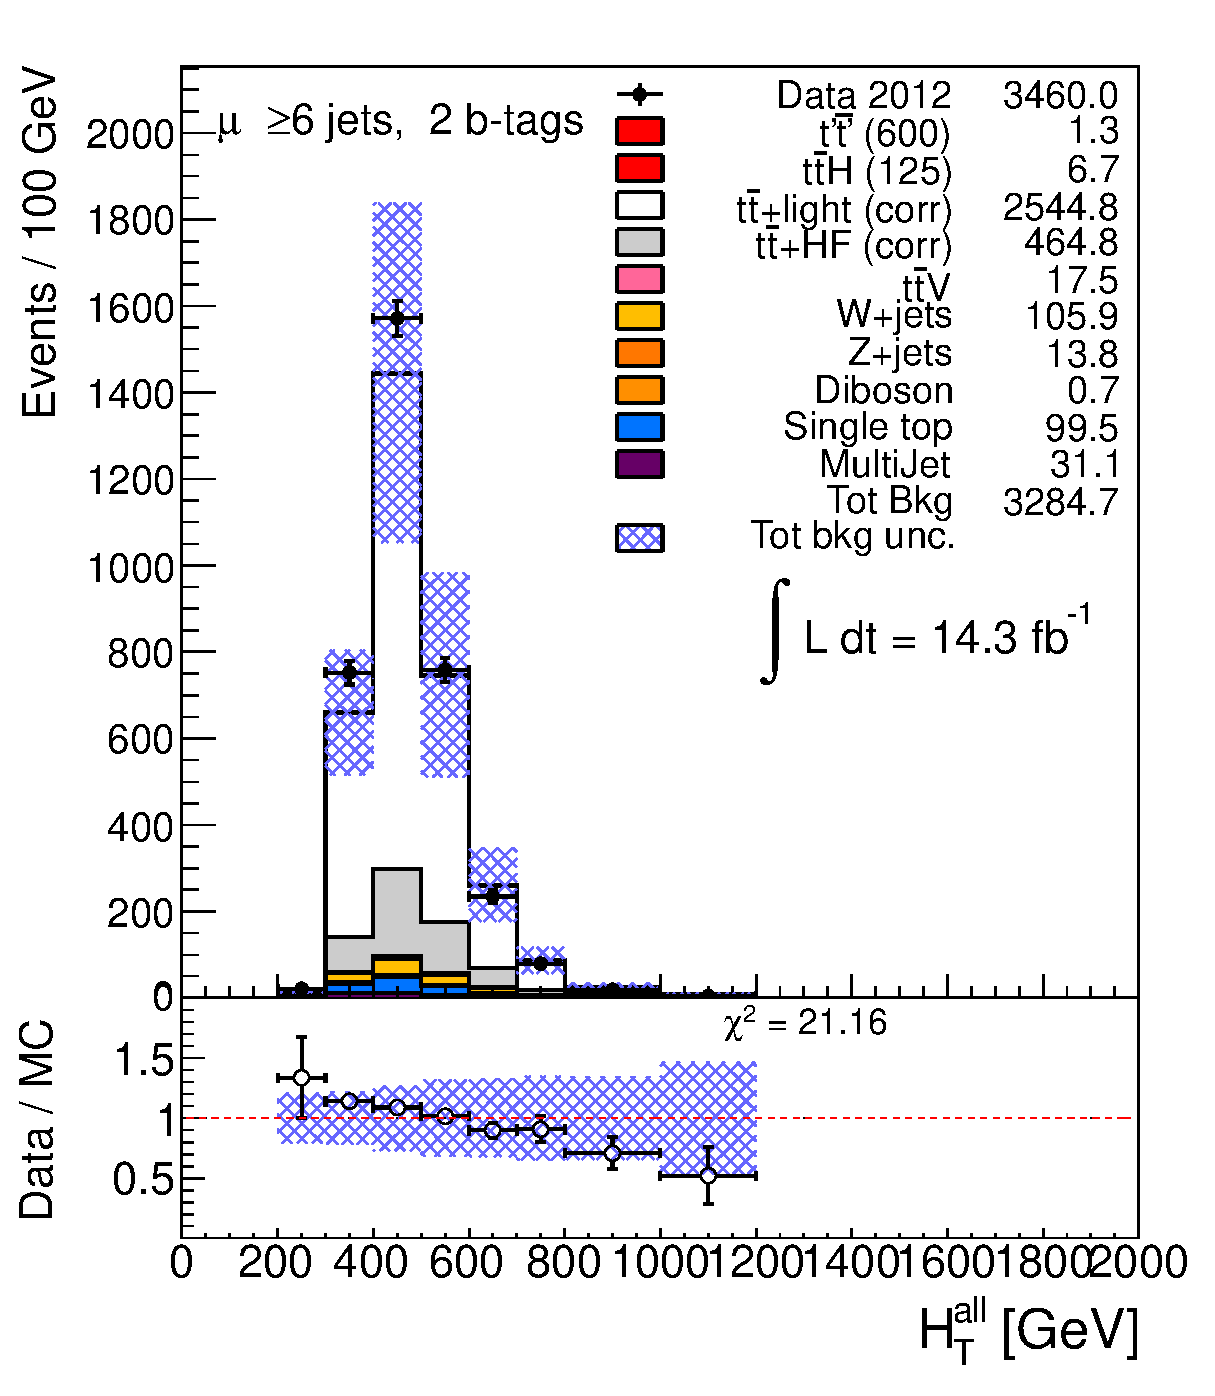
\includegraphics[width=0.30\textwidth]{figures/ht700SimpleBlindingCut/sysband_scaledAlpgen/HTAll_MUON_6jetin2btagex_NOMINAL.eps}  \\

\end{tabular}\caption{\small {Comparison between data and prediction in the $\mu$+jets channel in the control sample
with $\geq 6$ jets and $=2$ $b$-tagged jets  for a number of kinematic
variables. From top to bottom and left to right, the variables displayed are: lepton $\pt$, lepton $\eta$, missing transverse energy, $W$ transverse mass,
leading jet $\pt$, leading jet $\eta$,  $\hthad$ and $\HT$. The shaded area represents the total background uncertainty.}}
\label{fig:MUON_6jetin_2btagex}
\end{center}
\end{figure}
%%%%%%%%%%%%%%

\clearpage
%%%%%%%%%%%%%%
\begin{figure}[htbp]
\begin{center}
\begin{tabular}{ccc}
%
\includegraphics[width=0.30\textwidth]{figures/ht700SimpleBlindingCut/sysband_scaledAlpgen/LepPt_MUON_6jetin3btagex_NOMINAL.eps} &
\includegraphics[width=0.30\textwidth]{figures/ht700SimpleBlindingCut/sysband_scaledAlpgen/LepEta_MUON_6jetin3btagex_NOMINAL.eps} &
\includegraphics[width=0.30\textwidth]{figures/ht700SimpleBlindingCut/sysband_scaledAlpgen/MET_MUON_6jetin3btagex_NOMINAL.eps} \\
\includegraphics[width=0.30\textwidth]{figures/ht700SimpleBlindingCut/sysband_scaledAlpgen/Wlep_MassT_MUON_6jetin3btagex_NOMINAL.eps} &
\includegraphics[width=0.30\textwidth]{figures/ht700SimpleBlindingCut/sysband_scaledAlpgen/JetPt1_MUON_6jetin3btagex_NOMINAL.eps} &
\includegraphics[width=0.30\textwidth]{figures/ht700SimpleBlindingCut/sysband_scaledAlpgen/JetEta1_MUON_6jetin3btagex_NOMINAL.eps} \\
\includegraphics[width=0.30\textwidth]{figures/ht700SimpleBlindingCut/sysband_scaledAlpgen/Njets25_MUON_6jetin3btagex_NOMINAL.eps}  &
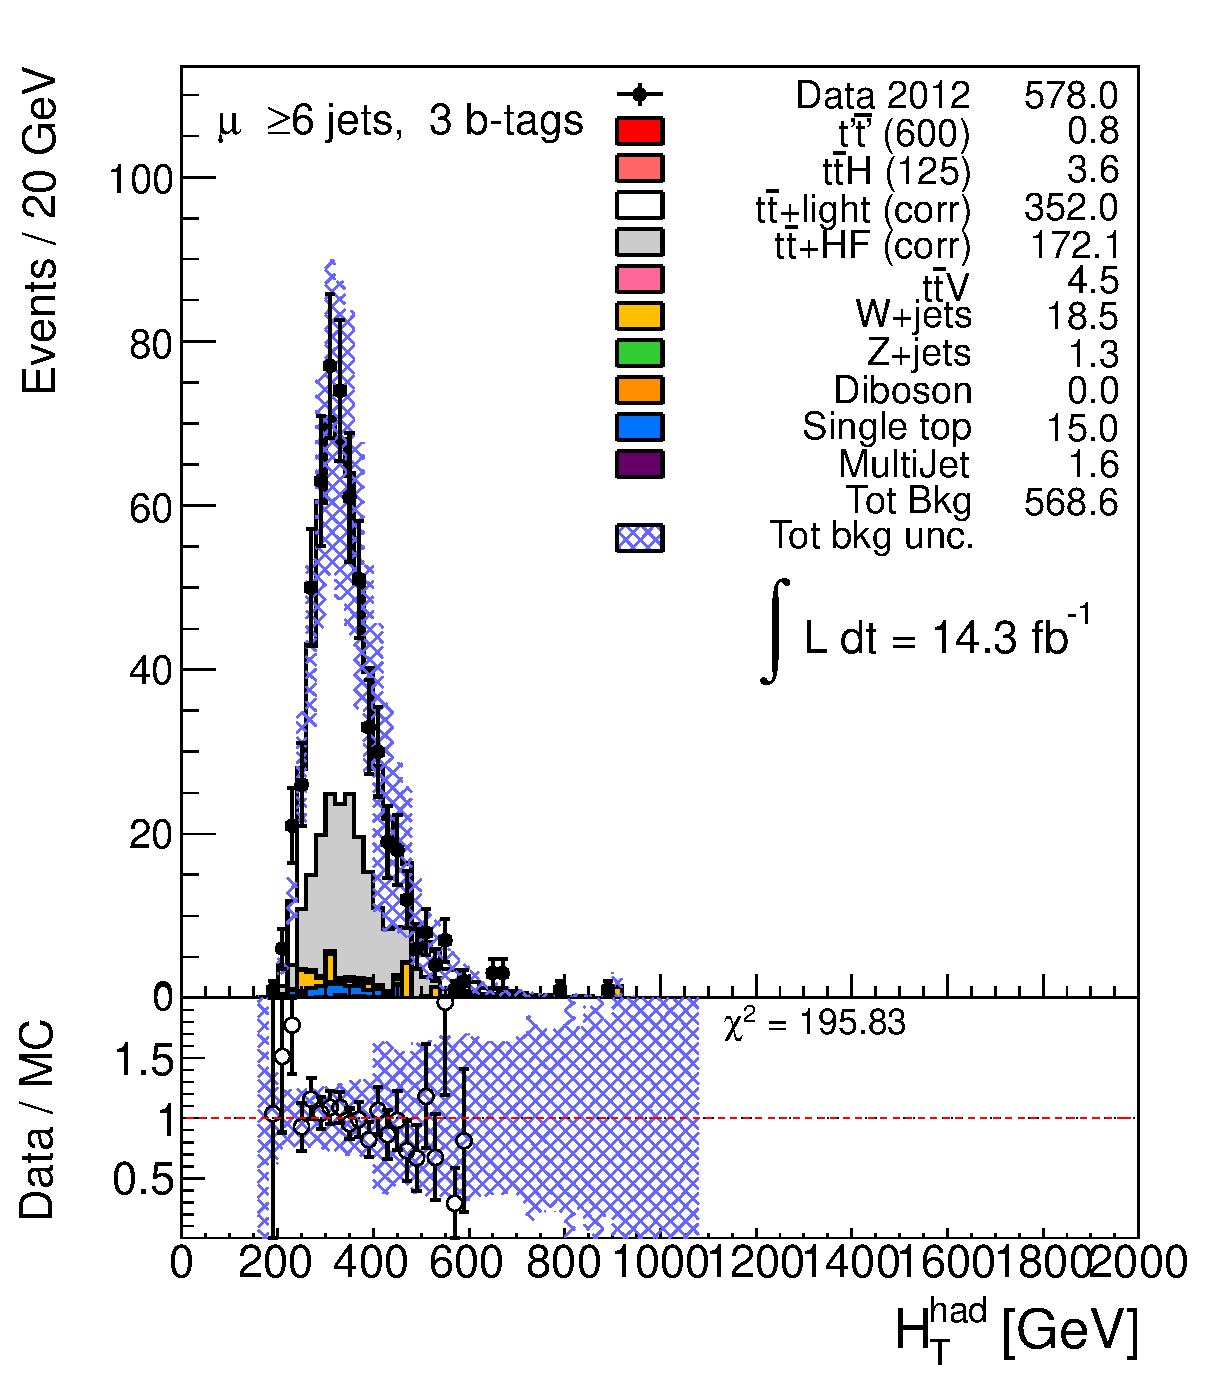
\includegraphics[width=0.30\textwidth]{figures/ht700SimpleBlindingCut/sysband_scaledAlpgen/HTHad_MUON_6jetin3btagex_NOMINAL.eps}  &
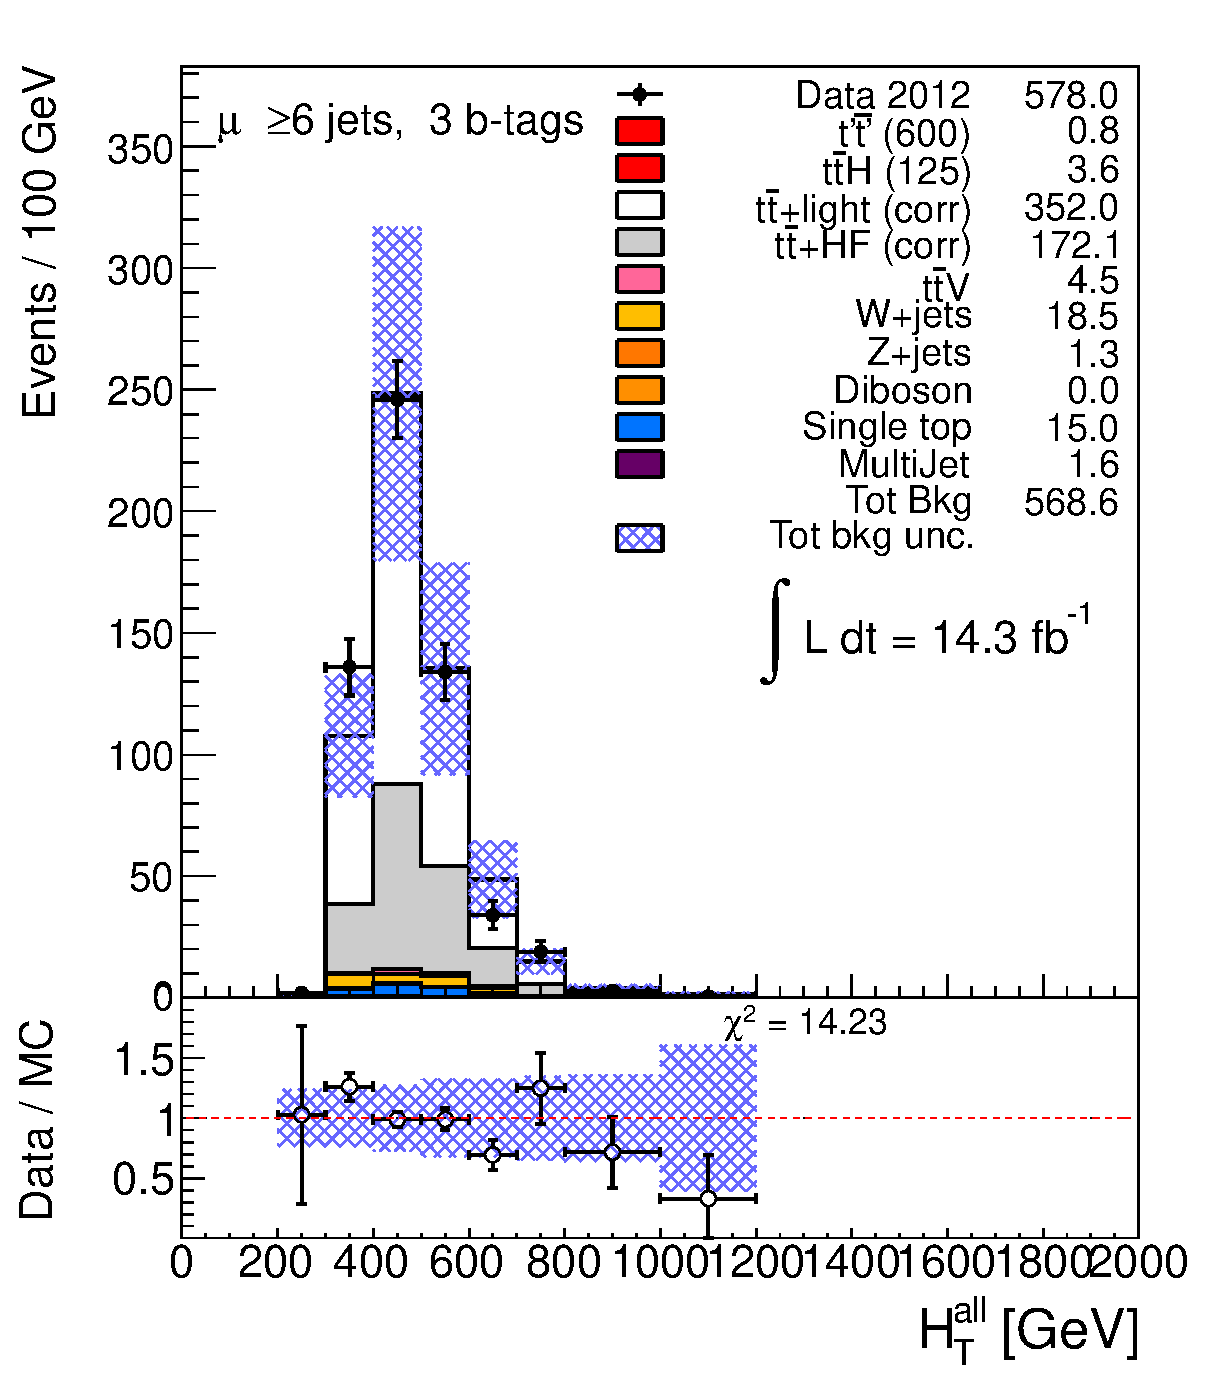
\includegraphics[width=0.30\textwidth]{figures/ht700SimpleBlindingCut/sysband_scaledAlpgen/HTAll_MUON_6jetin3btagex_NOMINAL.eps}  \\

\end{tabular}\caption{\small {Comparison between data and prediction in the $\mu$+jets channel in the control sample
with $\geq 6$ jets and $=3$ $b$-tagged jets  for a number of kinematic
variables. From top to bottom and left to right, the variables displayed are: lepton $\pt$, lepton $\eta$, missing transverse energy, $W$ transverse mass,
leading jet $\pt$, leading jet $\eta$,  $\hthad$ and $\HT$. The shaded area represents the total background uncertainty.}}
\label{fig:MUON_6jetin_3btagex}
\end{center}
\end{figure}
%%%%%%%%%%%%%%

\clearpage
%%%%%%%%%%%%%%
\begin{figure}[htbp]
\begin{center}
\begin{tabular}{ccc}
%
\includegraphics[width=0.30\textwidth]{figures/ht700SimpleBlindingCut/sysband_scaledAlpgen/LepPt_MUON_6jetin4btagin_NOMINAL.eps} &
\includegraphics[width=0.30\textwidth]{figures/ht700SimpleBlindingCut/sysband_scaledAlpgen/LepEta_MUON_6jetin4btagin_NOMINAL.eps} &
\includegraphics[width=0.30\textwidth]{figures/ht700SimpleBlindingCut/sysband_scaledAlpgen/MET_MUON_6jetin4btagin_NOMINAL.eps} \\
\includegraphics[width=0.30\textwidth]{figures/ht700SimpleBlindingCut/sysband_scaledAlpgen/Wlep_MassT_MUON_6jetin4btagin_NOMINAL.eps} &
\includegraphics[width=0.30\textwidth]{figures/ht700SimpleBlindingCut/sysband_scaledAlpgen/JetPt1_MUON_6jetin4btagin_NOMINAL.eps} &
\includegraphics[width=0.30\textwidth]{figures/ht700SimpleBlindingCut/sysband_scaledAlpgen/JetEta1_MUON_6jetin4btagin_NOMINAL.eps} \\
\includegraphics[width=0.30\textwidth]{figures/ht700SimpleBlindingCut/sysband_scaledAlpgen/Njets25_MUON_6jetin4btagin_NOMINAL.eps}  &
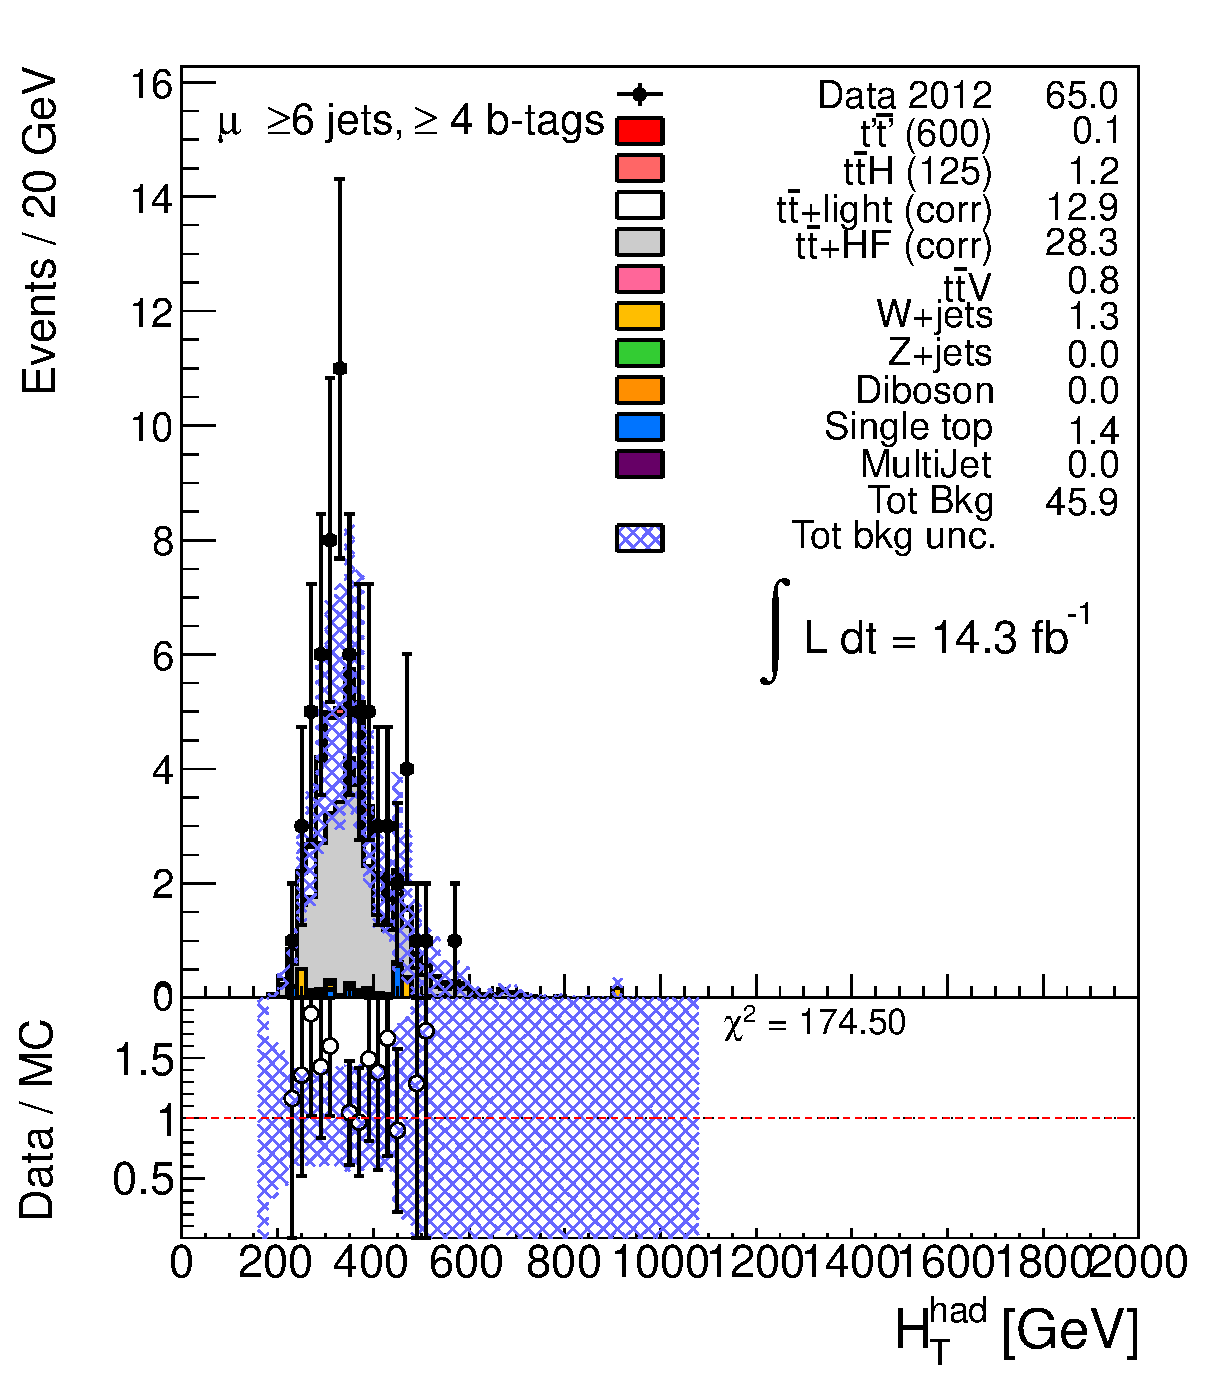
\includegraphics[width=0.30\textwidth]{figures/ht700SimpleBlindingCut/sysband_scaledAlpgen/HTHad_MUON_6jetin4btagin_NOMINAL.eps}  &
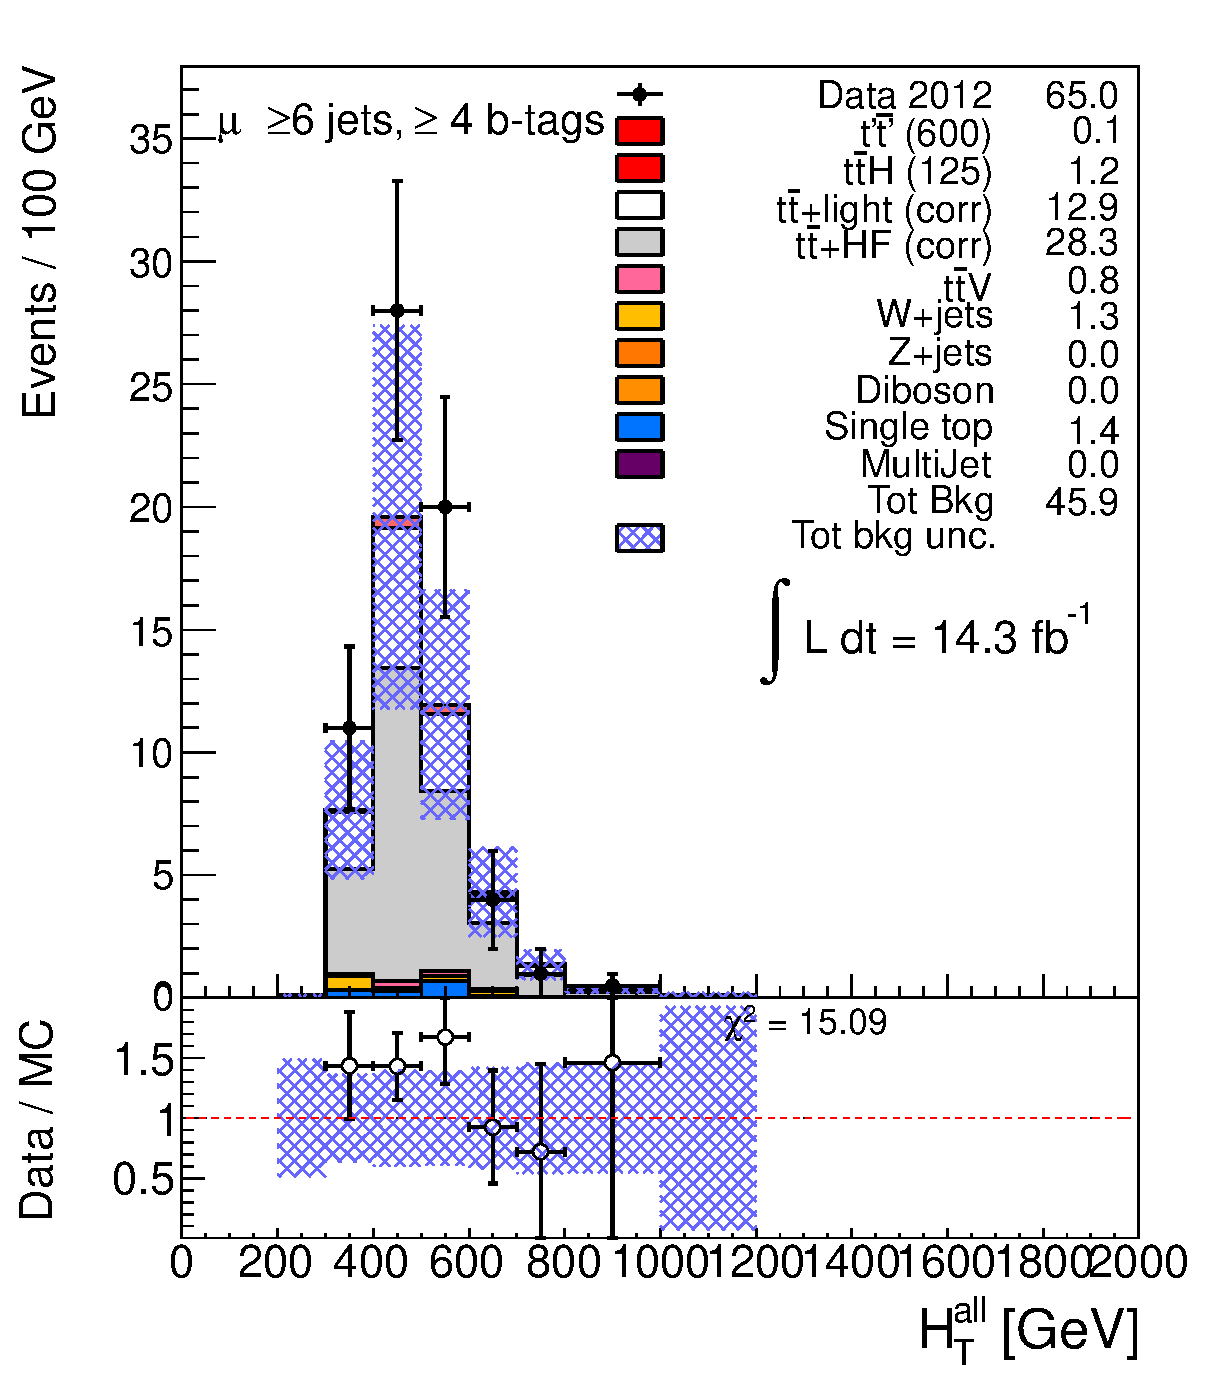
\includegraphics[width=0.30\textwidth]{figures/ht700SimpleBlindingCut/sysband_scaledAlpgen/HTAll_MUON_6jetin4btagin_NOMINAL.eps}  \\

\end{tabular}\caption{\small {Comparison between data and prediction in the $\mu$+jets channel in the control sample
with $\geq 6$ jets and $\geq 4$ $b$-tagged jets  for a number of kinematic
variables. From top to bottom and left to right, the variables displayed are: lepton $\pt$, lepton $\eta$, missing transverse energy, $W$ transverse mass,
leading jet $\pt$, leading jet $\eta$,  $\hthad$ and $\HT$. The shaded area represents the total background uncertainty.}}
\label{fig:MUON_6jetin_4btagin}
\end{center}
\end{figure}
%%%%%%%%%%%%%%
